\documentclass[a4paper]{article}

\usepackage[utf8]{inputenc}
\usepackage[T1]{fontenc}
\usepackage{textcomp}
\usepackage{amsmath, amssymb}
\usepackage{subcaption}
\usepackage{graphicx}
\usepackage{float}
\usepackage{hyperref}

% figure support
\usepackage{import}
\usepackage{xifthen}
\pdfminorversion=7
\usepackage{pdfpages}
\usepackage{transparent}
\newcommand{\incfig}[1]{%
    \def\svgwidth{\columnwidth}
    \import{./figures/}{#1.pdf_tex}
}

\pdfsuppresswarningpagegroup=1

\title{Statistical Methods in NLP 1\\
Assignment 1: Exploring Entropy and Language Modeling}
\date{\today}
\author{Andrew McIsaac}

\begin{document}
\maketitle
\tableofcontents

\section{Entropy of a Text}
\label{sec:entropy}

\subsection{English}

\begin{table}[H]
    \centering
    \caption{Conditional Entropy of English\\}
    \label{tab:en_entropy}
    \begin{tabular}{r|ccc|c}
        Text & & Entropy & & Avg. Perplexity \\
        \hline
        original & & 5.2874 & & 39.0553\\
        \hline
             & Min & Max & Average & \\
        \hline
        char {10\%} & 4.7262 & 4.7367 & 4.7308 & 26.5533 \\
        char {5\%} & 5.0522 & 5.0622 & 5.0564 & 33.2764 \\
        char {1\%} & 5.2473 & 5.2529 & 5.2504 & 38.0654 \\
        char {0.1\%} & 5.2825 & 5.2842 & 5.2835 & 38.9484 \\
        char {0.01\%} & 5.2868 & 5.2873 & 5.2871 & 39.0454 \\
        char {0.001\%} & 5.2874 & 5.2875 & 5.2874 & 39.0549 \\
        \hline
        word {10\%} & 5.4508 & 5.4602 & 5.4572 & 43.9313 \\
        word {5\%} & 5.3769 & 5.3836 & 5.3800 & 41.6440 \\
        word {1\%} & 5.3053 & 5.3087 & 5.3072 & 39.5928 \\
        word {0.1\%} & 5.2890 & 5.2899 & 5.2894 & 39.1089 \\
        word {0.01\%} & 5.2875 & 5.2878 & 5.2877 & 39.0609 \\
        word {0.001\%} & 5.2874 & 5.2876 & 5.2875 & 39.0560 \\
    \end{tabular}
\end{table}

\subsection{Czech}

\begin{table}[H]
    \centering
    \caption{Conditional Entropy of Czech\\}
    \label{tab:cz_entropy}
    \begin{tabular}{r|ccc|c}
        Text & & Entropy & & Avg. Perplexity \\
        \hline
        Original & &  4.7478 & & 26.8685 \\
        \hline
                 & Min & Max & Average & \\
        \hline
        char {10\%} & 3.9976 & 4.0117 & 4.0048 & 16.0534 \\
        char {5\%} & 4.3338 & 4.3443 & 4.3383 & 20.2283 \\
        char {1\%} & 4.6547 & 4.6610 & 4.6578 & 25.2430 \\
        char {0.1\%} & 4.7384 & 4.7399 & 4.7390 & 26.7039 \\
        char {0.01\%} & 4.7467 & 4.7471 & 4.7469 & 26.8516 \\
        char {0.001\%} & 4.7477 & 4.7478 & 4.7478 & 26.8671 \\
        \hline
        word {10\%} & 4.6335 & 4.6444 & 4.6378 & 24.8945 \\
        word {5\%} & 4.6965 & 4.7022 & 4.6992 & 25.9768 \\
        word {1\%} & 4.7383 & 4.7417 & 4.7394 & 26.7126 \\
        word {0.1\%} & 4.7464 & 4.7474 & 4.7468 & 26.8508 \\
        word {0.01\%} & 4.7475 & 4.7478 & 4.7477 & 26.8662 \\
        word {0.001\%} & 4.7478 & 4.7479 & 4.7478 & 26.8686 \\
    \end{tabular}
\end{table}

\begin{figure}[H]
	\centering
	\begin{subfigure}{0.49\textwidth}
		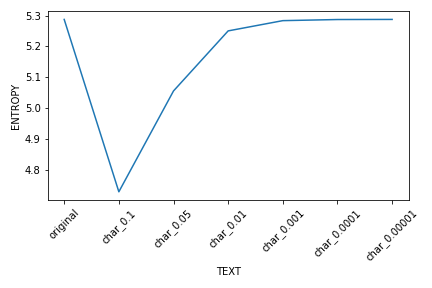
\includegraphics[width=\textwidth]{figures/en_char_entropy}
		\caption{English with messed up characters}
		\label{fig:en_char_entropy}
	\end{subfigure}
	\hfill
	\begin{subfigure}{0.49\textwidth}
		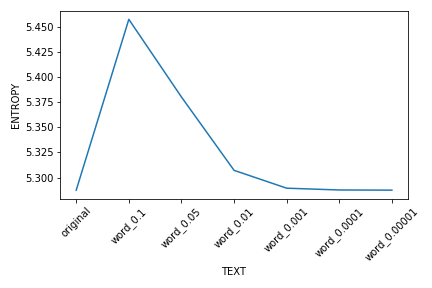
\includegraphics[width=\textwidth]{figures/en_word_entropy}
		\caption{English with messed up words}
		\label{fig:en_word_entropy}
	\end{subfigure}
	\hfill
	\begin{subfigure}{0.49\textwidth}
		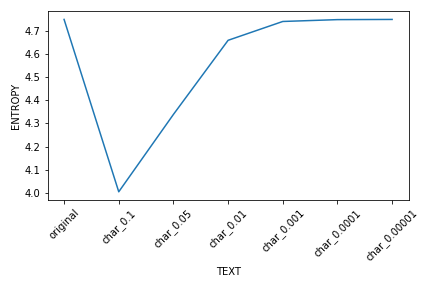
\includegraphics[width=\textwidth]{figures/cz_char_entropy}
		\caption{Czech with messed up characters}
		\label{fig:cz_char_entropy}
	\end{subfigure}
	\hfill
	\begin{subfigure}{0.49\textwidth}
		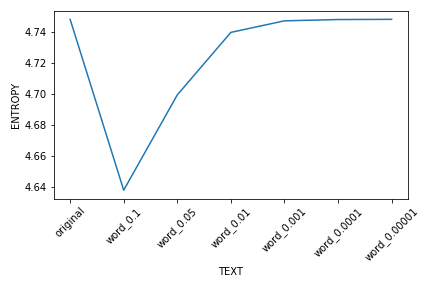
\includegraphics[width=\textwidth]{figures/cz_word_entropy}
		\caption{Czech with messed up words}
		\label{fig:cz_word_entropy}
	\end{subfigure}
	\caption{Conditional entropy of text for English and Czech with varying
		probabilities of messing up the text at the character and word level.}
	\label{fig:entropy}
\end{figure}

\subsection{Discussion}

\begin{table}[h]
	\centering
	\caption{Text statistics at word, bigram, and character level}
	\label{tab:stats}
	\begin{tabular}{r|cc}
	 & English & Czech \\
	 \hline
		Text Size & 221098 & 222412 \\
		Vocabulary Size & 9607 & 42826 \\
		Top 20 Word Frequency & 109798 & 78095 \\
		Unique Words & 3811 & 26315 \\
		\hline
		Different Bigrams & 73246 & 147136 \\
		Unique Bigrams & 49600 & 125007 \\
		\hline
		Total Characters & 972917 & 1030631 \\
		Average Characters & 4.400 & 4.633 \\
		Different Characters & 74 & 117 \\
	\end{tabular}
\end{table}

The conditional entropy of the original Czech data is lower than the original
English data (4.7478 compared to 5.2874). This suggests that the ability to
predict a word given another word is slightly better for Czech. From Table
\ref{tab:stats}, comparing vocabulary size shows that the number of different
words in Czech is about 4.5x more than in English, meaning that there are more
different bigrams for Czech (about 2x). Further, the number of unique bigrams
in Czech represents a larger proportion (85.0\%) of the total different bigrams
when compared to English (67.7\%). This means that 85\% of the bigrams have
perfect conditional predictive ability, and do not increase the entropy at all.
So the total conditional entropy of Czech is lower than English. The reason for
the difference in the distribution between languages may be because of the
morphological richness of Czech, with many inflectional forms that English does
not have contributing to the larger vocabulary.

For both English and Czech data, when messing up characters within words, the
entropy changes in a similar pattern (Figs. \ref{fig:en_char_entropy},
\subref{fig:cz_char_entropy}). For very small probabilities the entropy is
approximately equal to the original text, but as the probability of messing up a
character increases, the entropy decreases. Again, this may be because the
number of hapax legomena (words occurring only once in the text) increases and
thus the number of unique bigrams, meaning fewer bigrams have any uncertainty at
all.

When messing up words, however, the conditional entropy of English increases
at larger probabilities, while for Czech it decreases (Figs.
\ref{fig:en_word_entropy}, \subref{fig:cz_word_entropy}). A large reason for
this may be because of the respective vocabulary sizes, and specifically the
hapax legomena. The number of hapax legomena reduce quite significantly in
English because of the smaller vocabulary, so that when changing a word with
some probability in two similar sized texts, the hapax legomena are chosen more
often and are no longer unique. Hence the log conditional probability of a
bigram is 0 less often, and this results in an increase in conditional entropy.
For Czech, this effect isn't seen to the same extent because there are far more
hapax legomena, (26315 vs 3811), and so there are still many 0 terms which keep
the conditional entropy down.

Finally, the range in which the entropy changes differs when messing up
characters or words. The conditional entropy has a range of 0.56 for English and
0.74 for Czech for characters, while for words it is just 0.17 and 0.11 for
English and Czech respectively. This emphasises the importance of hapax legomena
in determining the entropy, with changing characters making many more unique
words.

\subsection{Independent Languages $L_1$ and $L_2$}
Assuming that texts $T_1$ and $T_2$ have start and end tags, so that the bigram
count of the final word of $T_1$ is not affected by appending $T_2$, the
conditional entropy of the joined text will be greater than the individual
entropies $E$ of $T_1$ and $T_2$. This is because the conditional probabilities
of the entropy equation do not change, and the joint probabilities, as computed
by MLE, only change in their denominator, which is equal to the sum of the
number of bigrams in the text minus one (accounting for the reduced number of
bigrams including start/end tags). So with a smaller denominator and the same
numerator over all pairs of words, the total conditional entropy is larger than
$E$.

\section{Cross-Entropy and Language Modeling}
\label{sec:lm}

\subsection{Smoothing Parameters}
Trained smoothing parameters using both heldout and training data for both
languages are detailed in Table \ref{tab:smoothing}.

\begin{table}[h]
	\centering
	\caption{Smoothing parameters computed with the EM algorithm with
		terminating condition $\epsilon=0.00001$}
	\label{tab:smoothing}
	\begin{tabular}{c|cccc}
		Data & l\_0 & l\_1 & l\_2 & l\_3 \\
		\hline
		EN Heldout & 0.0700 & 0.2539 & 0.4922 & 0.1836 \\
		EN Train & 7.504e-29 & 1.365e-14 & 5.181e-06 & 0.9999 \\
		\hline
		CZ Heldout & 0.1402& 0.4289& 0.2446 & 0.1862 \\
		CZ Train & 1.717e-42 & 1.110e-21 & 3.524e-06 & 0.9999 \\
	\end{tabular}
\end{table}

\subsection{Cross-Entropy}
Cross-entropy for all permutations, along with the associated smoothing
lambda parameters, are found for English in Table \ref{tab:ce_en}, and for Czech
in Table \ref{tab:ce_cz}. 

\begin{table}[h]
	\centering
	\caption{Cross-entropy on English test data with different smoothing
	parameters}
	\label{tab:ce_en}
	\begin{tabular}{r|cccc|c}
		Text & \multicolumn{4}{|c|}{Lambdas} & Cross-Entropy \\
		\hline
			 & l\_0 & l\_1 & l\_2 & l\_3 & \\
		\hline
		original & 0.0700 & 0.2539 & 0.4922 & 0.1836 & 7.4677\\
		\hline
		add {10\%}  & 0.0630 & 0.2285 & 0.4430 & 0.2652 & 7.4693\\
		add {20\%}  & 0.0560 & 0.2031 & 0.3938 & 0.3469 & 7.4962\\
		add {30\%}  & 0.0490 & 0.1777 & 0.3445 & 0.4285 & 7.546\\
		add {40\%}  & 0.0420 & 0.1523 & 0.2953 & 0.5101 & 7.6197\\
		add {50\%}  & 0.0350 & 0.1269 & 0.2461 & 0.5918 & 7.7215\\
		add {60\%}  & 0.0280 & 0.1015 & 0.1969 & 0.6734 & 7.8602\\
		add {70\%}  & 0.0210 & 0.0761 & 0.1476 & 0.7550 & 8.0533\\
		add {80\%}  & 0.0140 & 0.0507 & 0.0984 & 0.8367 & 8.3409\\
		add {90\%}  & 0.0070 & 0.0253 & 0.0492 & 0.9183 & 8.8501\\
		add {95\%} & 0.0035 & 0.0127 & 0.0246 & 0.9592 & 9.3614\\
		add {99\%} & 0.0007 & 0.0025 & 0.0049 & 0.9918 & 10.5003\\
		\hline
		discount {90\%} & 0.0716 & 0.2597 & 0.5033 & 0.1652 & 7.4716\\
		discount {80\%} & 0.0732 & 0.2654 & 0.5144 & 0.1469 & 7.4773\\
		discount {70\%} & 0.0748 & 0.2711 & 0.5254 & 0.1285 & 7.4851\\
		discount {60\%} & 0.0763 & 0.2768 & 0.5365 & 0.1101 & 7.4954\\
		discount {50\%} & 0.0779 & 0.2825 & 0.5476 & 0.0918 & 7.5086\\
		discount {40\%} & 0.0795 & 0.2882 & 0.5587 & 0.0734 & 7.5255\\
		discount {30\%} & 0.0811 & 0.2939 & 0.5697 & 0.0550 & 7.5471\\
		discount {20\%} & 0.0826 & 0.2997 & 0.5808 & 0.0367 & 7.5758\\
		discount {10\%} & 0.0842 & 0.3054 & 0.5919 & 0.0183 & 7.6166\\
		discount {0\%}  & 0.0858 & 0.3111 & 0.6030 & 0      & 7.7035\\
	\end{tabular}
\end{table}

\begin{table}[H]
	\centering
	\caption{Cross-entropy on Czech test data with different smoothing
	parameters}
	\label{tab:ce_cz}
	\begin{tabular}{r|cccc|c}
		Text & \multicolumn{4}{|c|}{Lambdas} & Cross-Entropy \\
		\hline
			 & l\_0 & l\_1 & l\_2 & l\_3 & \\
		\hline
		original & 0.1402 & 0.4289 & 0.2446 & 0.1862 & 10.2198\\
		\hline
		add {10\%} & 0.1262 & 0.3860 & 0.2201 & 0.2675 & 10.2243\\
		add {20\%} & 0.1121 & 0.3431 & 0.1956 & 0.3489 & 10.2538\\
		add {30\%} & 0.0981 & 0.3002 & 0.1712 & 0.4303 & 10.3059\\
		add {40\%} & 0.0841 & 0.2573 & 0.1467 & 0.5117 & 10.3817\\
		add {50\%} & 0.0701 & 0.2144 & 0.1223 & 0.5930 & 10.4852\\
		add {60\%} & 0.0560 & 0.1715 & 0.0978 & 0.6744 & 10.6250\\
		add {70\%} & 0.0420 & 0.1286 & 0.0733 & 0.7558 & 10.8180\\
		add {80\%} & 0.0280 & 0.0857 & 0.0489 & 0.8372 & 11.1027\\
		add {90\%} & 0.0140 & 0.0428 & 0.0244 & 0.9186 & 11.6002\\
		add {95\%} & 0.0070 & 0.0214 & 0.0122 & 0.9593 & 12.0925\\
		add {99\%} & 0.0014 & 0.0042 & 0.0024 & 0.9918 & 13.1646\\
		\hline
		discount {90\%} & 0.1434 & 0.4387 & 0.2502 & 0.1675 & 10.2230\\
		discount {80\%} & 0.1466 & 0.4485 & 0.2558 & 0.1489 & 10.2281\\
		discount {70\%} & 0.1498 & 0.4583 & 0.2614 & 0.1303 & 10.2353\\
		discount {60\%} & 0.1530 & 0.4681 & 0.2669 & 0.1117 & 10.2451\\
		discount {50\%} & 0.1562 & 0.4780 & 0.2725 & 0.0930 & 10.2578\\
		discount {40\%} & 0.1595 & 0.4878 & 0.2781 & 0.0744 & 10.2743\\
		discount {30\%} & 0.1627 & 0.4976 & 0.2837 & 0.0558 & 10.2959\\
		discount {20\%} & 0.1659 & 0.5074 & 0.2893 & 0.0372 & 10.3250\\
		discount {10\%} & 0.1691 & 0.5172 & 0.2949 & 0.0186 & 10.3679\\
		discount {0\%}  & 0.1723 & 0.5270 & 0.3005 & 0      & 10.4885\\
	\end{tabular}
\end{table}

\begin{figure}[H]
	\centering
	\begin{subfigure}{\textwidth}
		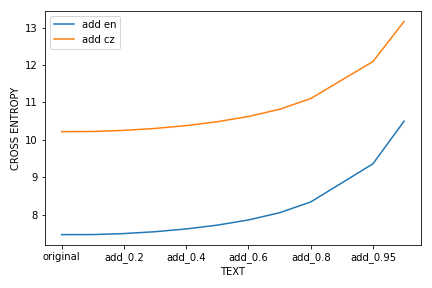
\includegraphics[width=\textwidth]{figures/add_lm.png}
		\caption{l\_3 boosted}
		\label{fig:add_lm}
	\end{subfigure}
	\hfill
	\begin{subfigure}{\textwidth}
		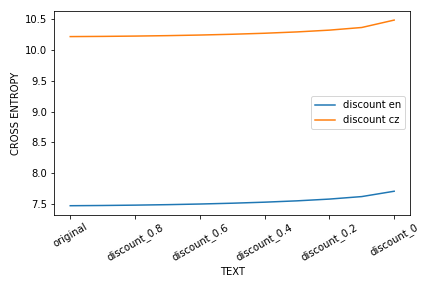
\includegraphics[width=\textwidth]{figures/discount_lm.png}
		\caption{l\_3 discounted}
		\label{fig:discount_lm}
	\end{subfigure}
	\caption{Cross-entropy of English and Czech data with a modified l\_3
	parameter}
	\label{fig:tweaked_lm}
\end{figure}

Figure \ref{fig:tweaked_lm} shows how the cross-entropy changes as the smoothing
parameters change. It can be seen that the cross-entropy is lowest for the
original trained lambdas for both languages, and in both adding and discounting
the l\_3 parameter. This would be expected to be the case, as the trained
lambdas represent the optimal values for the heldout data, so assuming a similar
distribution between heldout and test data means that the original lambdas are
close to optimal for the test data.

The cross-entropy for Czech is higher than it is for English. This suggests that
the distribution learnt by the training algorithm is closer to that found in the
test data. It can be seen that for English the coverage of words in the test
data that have been seen in the training data is 75.8\%, while for Czech it is
just 65.2\%. As seen in Table \ref{tab:stats}, the reason for this may again be
because of the higher number of unique words in Czech arising from its rich
morphology.

\appendix

\section{Code and Results Files}
\label{sec:code}

Note that \texttt{numpy} is required to run the code.

The code for Section \ref{sec:entropy} is in the file \texttt{entropy.py}.
Running the file with \texttt{python entropy.py} will run the entire code for
two text files called \texttt{TEXTEN1.txt} and \texttt{TEXTCZ1.txt}. The results
of all experiments will be saved in files called \texttt{entropy\_resultsEN.txt}
and \texttt{entropy\_resultsCZ.txt} respectively.

The code for Section \ref{sec:lm} is in the file \texttt{lm.py}. Running the
file with \texttt{python lm.py} will run the entire code for two text files
called \texttt{TEXTEN1.txt} and \texttt{TEXTCZ1.txt}. The results of all
experiments will be saved in files called \texttt{lm\_resultsEN.txt} and
\texttt{lm\_resultsCZ.txt} respectively.

\end{document}
